\documentclass[12pt, a4paper, oneside]{ctexart}
\usepackage{amsmath, amsthm, amssymb, bm, color, framed, graphicx, hyperref, mathrsfs}

\title{\textbf{3月9日作业}}
\author{韩岳成 524531910029}
\date{\today}
\linespread{1.5}
\definecolor{shadecolor}{RGB}{241, 241, 255}
\newcounter{problemname}
\newenvironment{problem}{\begin{shaded}\stepcounter{problemname}\par\noindent\textbf{题目\arabic{problemname}. }}{\end{shaded}\par}
\newenvironment{solution}{\par\noindent\textbf{解答. }}{\par}
\newenvironment{note}{\par\noindent\textbf{题目\arabic{problemname}的注记. }}{\par}
\everymath{\displaystyle}

\begin{document}

\maketitle

\begin{problem}
    证明：任何简单图必有至少两个顶点具有相等的度.
\end{problem}

\begin{solution}
    反证假设存在一个简单图 $G$，其所有顶点的度数都不相等。设 $G$ 有 $n(n\ge 2)$ 个顶点，则这些顶点的度数只能依次为 $0, 1, 2, \ldots, n-1$，共 $n$ 个不同的数值。

    但此时我们注意到同时存在度数为 $0$ 和度数为 $n-1$ 的顶点，这意味着有一个顶点与所有其他顶点相连，而另一个顶点与任何其他顶点都不相连，这显然是矛盾的。因此，度数为 $0$ 和度数为 $n-1$ 的顶点不能同时存在，假设不成立。因此任何简单图必有至少两个顶点具有相等的度。
\end{solution}

\begin{problem}
    证明：如果图 G 不连通，则其补图 $\bar{G}$ 必连通.
\end{problem}

\begin{solution}
    设图 $G$ 有 $n$ 个顶点，且不连通。则 $G$ 至少有两个连通分支。

    任取 $\bar{G}$ 中的两个不同顶点 $u$ 和 $v$。如果在 $\bar{G}$ 中它们之间有边，则结论成立。否则，在 $G$ 中它们之间有边，则 $u$ 和 $v$ 处于同一连通分支之中。

    由于 $G$ 不连通，存在一个顶点 $w$，使得它与 $u$ 与 $v$ 在不同的连通分支中。那么在 $\bar{G}$ 中，$(u, w)$ 和 $(w, v)$ 都有边，因此存在一条从 $u$ 到 $v$ 的路径。

    因此，$\bar{G}$ 是连通的。
\end{solution}

\begin{problem}
讨论下列三个图的同构性.
\begin{center}
    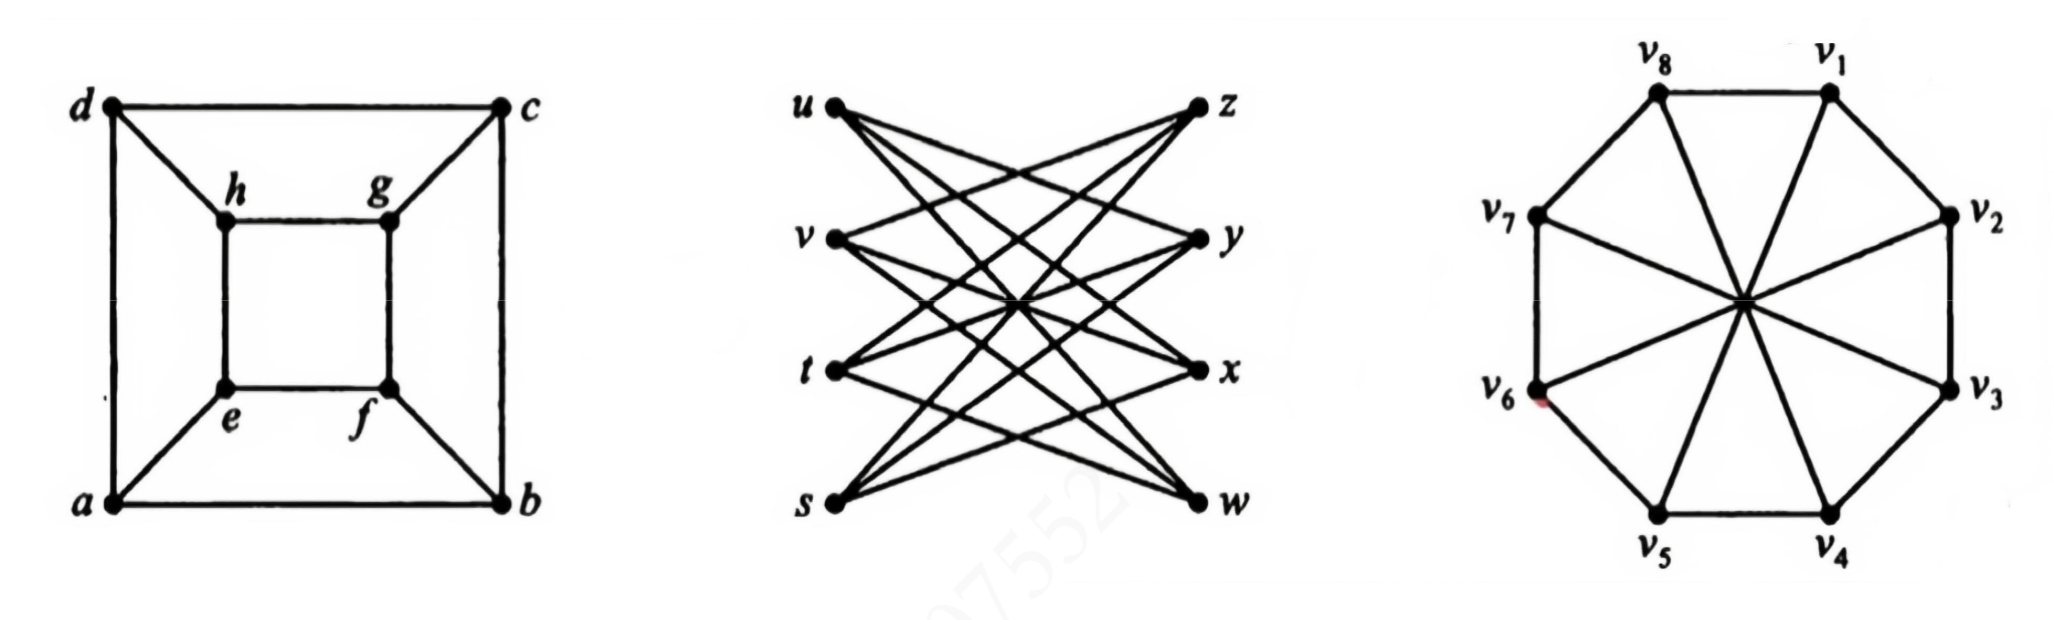
\includegraphics[width=0.8\textwidth]{3.png}
\end{center}
\end{problem}

\begin{solution}
对于图1和图2，我们可以通过以下映射来证明它们同构：
\[
\begin{aligned}
a \leftrightarrow u,\,
b \leftrightarrow y,\,
c \leftrightarrow t,\,
d \leftrightarrow w,\,
e \leftrightarrow x,\,
f \leftrightarrow s,\,
g \leftrightarrow z,\,
h \leftrightarrow v.
\end{aligned}
\]
经检验，对于图1中的任意两点 $x_1, x_2$，它们在图1中相邻当且仅当它们在映射下的像 $f(x_1), f(x_2)$ 在图2中相邻（例如：$a$ 在图1中连接 $b, d, e$；对应的 $u$ 在图2中连接 $y, w, x$，依此类推全部吻合）。因此该双射保持了邻接关系，图1和图2同构。

对于图2和图3，由于图2为一个二部图，因此图2不存在奇环。但图3中存在长度为5的奇环（例如：$v_1 - v_2 - v_3 - v_4 - v_5 - v_1$），因此图2和图3不可能同构。

因此，图1和图2同构，而图3与它们都不相同。
\end{solution}

\begin{problem}
若 $G$ 是简单图且 $\delta(G) \geq k$，则 $G$ 有长为至少 $k$ 的路；如果 $k \geq 2$，则 $G$ 还包含一个长至少为 $k + 1$ 的圈.
\end{problem}

\begin{solution}
    设 $G$ 是一个简单图，且 $\delta(G) \geq k$。我们首先证明 $G$ 中存在一条长度至少为 $k$ 的路径.

    选择 $G$ 中的一条最长路径 $P (v_1, v_2, \ldots, v_n)$. 由于 $P$ 是最长路径，因此 $v_1$ 和 $v_n$ 的所有邻居都必须在路径 $P$ 上，否则我们可以通过连接 $v_1$ 或 $v_n$ 与一个不在路径上的邻居来构造一条更长的路径，这与 $P$ 的最长性质矛盾。由于 $\delta(G) \geq k$，每个顶点至少有 $k$ 个邻居，且$v_1$的所有邻居都在路径 $P$ 上，因此路径 $P$ 上至少有 $k+1$ 个顶点，长度至少为 $k$。

    接下来，我们证明如果 $k \geq 2$，则 $G$ 中还包含一个长度至少为 $k + 1$ 的圈。

    由于 $P(v_1, \dots, v_n)$ 是最长路径，$v_1$ 的所有邻居都在 $P$ 上。因为 $\delta(G) \ge k$，$v_1$ 在 $P$ 上的邻居至少有 $k$ 个。

    设 $v_1$ 在路径 $P$ 上最远的那个邻居是 $v_m$。
    因为 $v_1$ 本身是路径的第 1 个点，它后面至少跟着 $k$ 个它的邻居，所以最远的邻居 $v_m$ 的下标 $m$ 必须满足 $m \ge k + 1$。
    此时，我们利用路径 $P$ 上从 $v_1$ 到 $v_m$ 的这一段子路径，加上边 $(v_m, v_1)$，就构成了一个圈：
    \[v_1 - v_2 - v_3 - \dots - v_m - v_1\]
    这个圈的顶点数量为 $m$，因为 $m \ge k+1$，所以这个圈的长度至少为 $k+1$。证毕。”
\end{solution}

\begin{problem}
设 G 是一个简单图. 证明：若 $\text{diam}\,G \ge 3$，则 $\text{diam}\,\bar{G} \le 3$；若$\text{rad}\,G \ge 3$，则 $\text{rad}\,\bar{G} \le 2$.
\end{problem}

\begin{solution}
    \noindent\textbf{第一部分：证明 若 $\text{diam}\,G \ge 3$，则 $\text{diam}\,\bar{G} \le 3$}

    因为 $\text{diam}\,G \ge 3$，所以 $G$ 中必定存在两顶点 $u, v \in V(G)$，使得 $d_G(u, v) \ge 3$。由此可以得出，$u$ 和 $v$ 在 $G$ 中不相邻，在 $\bar{G}$ 中$u$ 和 $v$ 相邻。且 $u$ 和 $v$ 在 $G$ 中没有共同的邻接点（否则存在路径 $u-w-v$，使得 $d_G(u,v) \le 2$）。这意味着，对于任意顶点 $w \in V(G)$，它在 $G$ 中不可能同时与 $u$ 和 $v$ 相邻。换言之，在补图 $\bar{G}$ 中，任意顶点 $w$ 必然至少与 $u$ 或 $v$ 之一相邻。

现任取 $V(G)$ 中任意两个不同的顶点 $x$ 和 $y$，讨论它们在 $\bar{G}$ 中的距离 $d_{\bar{G}}(x, y)$：
\begin{itemize}
    \item \textbf{情形 1：} 若 $(x,y)\notin E(G)$。
    则在补图中 $(x,y) \in E(\bar{G})$，故 $d_{\bar{G}}(x, y) = 1 \le 3$。
    
    \item \textbf{情形 2：} 若 $(x,y) \in E(G)$。
    根据前述推论，在 $\bar{G}$ 中，$x$ 必与 $u$ 或 $v$ 之一相邻；同理，$y$ 也必与 $u$ 或 $v$ 之一相邻。
    \begin{itemize}
        \item 若 $x$ 和 $y$ 在 $\bar{G}$ 中与同一个顶点（不妨设为 $u$）相邻，则在 $\bar{G}$ 中存在路径 $x-u-y$，故 $d_{\bar{G}}(x, y) \le 2 \le 3$。
        \item 若 $x$ 和 $y$ 在 $\bar{G}$ 中与不同的顶点相邻（不妨设 $x$ 与 $u$ 相邻，$y$ 与 $v$ 相邻），由推论(1)知 $(u,v) \in E(\bar{G})$。则在 $\bar{G}$ 中存在路径 $x-u-v-y$，故 $d_{\bar{G}}(x, y) \le 3$。
    \end{itemize}
\end{itemize}
综上所述，对于任意 $x, y \in V(G)$，均有 $d_{\bar{G}}(x, y) \le 3$。因此，$\text{diam}\,\bar{G} \le 3$。

\vspace{1em}
\noindent\textbf{第二部分：证明 若 $\text{rad}\,G \ge 3$，则 $\text{rad}\,\bar{G} \le 2$}

若 $\text{rad}\,G \ge 3$，意味着对图 $G$ 中的任意顶点 $v \in V(G)$，其离心率 $e_G(v) \ge 3$。即必存在一顶点 $u \in V(G)$，使得 $d_G(v, u) \ge 3$。

我们来考查任意选定的顶点 $v$ 在补图 $\bar{G}$ 中的离心率 $e_{\bar{G}}(v)$。任取图中另一顶点 $x \in V(G)$：
\begin{itemize}
    \item 若 $(v,x) \notin E(G)$。
    则在补图中 $(v,x) \in E(\bar{G})$，故 $d_{\bar{G}}(v, x) = 1 \le 2$。
    
    \item 若 $(v,x) \in E(G)$。
    因为 $d_G(v, u) \ge 3$，若 $x$ 在 $G$ 中与 $u$ 相邻，则存在路径 $v-x-u$ 长度为 2，与 $d_G(v, u) \ge 3$ 矛盾。因此，$x$ 在 $G$ 中必不与 $u$ 相邻，即 $(x,u) \notin E(G)$。
    转至补图 $\bar{G}$ 中，这意味着 $(x,u) \in E(\bar{G})$。同时，由 $d_G(v, u) \ge 3$ 可知 $(v,u) \notin E(G)$，即 $(v,u) \in E(\bar{G})$。
    因此，在补图 $\bar{G}$ 中存在路径 $v-u-x$，故 $d_{\bar{G}}(v, x) \le 2$。
\end{itemize}

这表明，对于任意顶点 $v$，它到其他任意顶点 $x$ 在 $\bar{G}$ 中的距离都不超过 2，即 $e_{\bar{G}}(v) \le 2$。
因为图的半径是所有顶点离心率的最小值，即 $\text{rad}\,\bar{G} = \min_{v \in V} e_{\bar{G}}(v)$，既然所有顶点的离心率均不超过 2，显然有 $\text{rad}\,\bar{G} \le 2$。

\hfill $\blacksquare$
\end{solution}
\end{document}
